% Options for packages loaded elsewhere
\PassOptionsToPackage{unicode}{hyperref}
\PassOptionsToPackage{hyphens}{url}
\PassOptionsToPackage{dvipsnames,svgnames*,x11names*}{xcolor}
%
\documentclass[
]{article}
\usepackage{lmodern}
\usepackage{amssymb,amsmath}
\usepackage{ifxetex,ifluatex}
\ifnum 0\ifxetex 1\fi\ifluatex 1\fi=0 % if pdftex
  \usepackage[T1]{fontenc}
  \usepackage[utf8]{inputenc}
  \usepackage{textcomp} % provide euro and other symbols
\else % if luatex or xetex
  \usepackage{unicode-math}
  \defaultfontfeatures{Scale=MatchLowercase}
  \defaultfontfeatures[\rmfamily]{Ligatures=TeX,Scale=1}
\fi
% Use upquote if available, for straight quotes in verbatim environments
\IfFileExists{upquote.sty}{\usepackage{upquote}}{}
\IfFileExists{microtype.sty}{% use microtype if available
  \usepackage[]{microtype}
  \UseMicrotypeSet[protrusion]{basicmath} % disable protrusion for tt fonts
}{}
\makeatletter
\@ifundefined{KOMAClassName}{% if non-KOMA class
  \IfFileExists{parskip.sty}{%
    \usepackage{parskip}
  }{% else
    \setlength{\parindent}{0pt}
    \setlength{\parskip}{6pt plus 2pt minus 1pt}}
}{% if KOMA class
  \KOMAoptions{parskip=half}}
\makeatother
\usepackage{xcolor}
\IfFileExists{xurl.sty}{\usepackage{xurl}}{} % add URL line breaks if available
\IfFileExists{bookmark.sty}{\usepackage{bookmark}}{\usepackage{hyperref}}
\hypersetup{
  pdftitle={Course title},
  colorlinks=true,
  linkcolor=Maroon,
  filecolor=Maroon,
  citecolor=Blue,
  urlcolor=blue,
  pdfcreator={LaTeX via pandoc}}
\urlstyle{same} % disable monospaced font for URLs
\usepackage[margin=1in]{geometry}
\usepackage{color}
\usepackage{fancyvrb}
\newcommand{\VerbBar}{|}
\newcommand{\VERB}{\Verb[commandchars=\\\{\}]}
\DefineVerbatimEnvironment{Highlighting}{Verbatim}{commandchars=\\\{\}}
% Add ',fontsize=\small' for more characters per line
\usepackage{framed}
\definecolor{shadecolor}{RGB}{248,248,248}
\newenvironment{Shaded}{\begin{snugshade}}{\end{snugshade}}
\newcommand{\AlertTok}[1]{\textcolor[rgb]{0.94,0.16,0.16}{#1}}
\newcommand{\AnnotationTok}[1]{\textcolor[rgb]{0.56,0.35,0.01}{\textbf{\textit{#1}}}}
\newcommand{\AttributeTok}[1]{\textcolor[rgb]{0.77,0.63,0.00}{#1}}
\newcommand{\BaseNTok}[1]{\textcolor[rgb]{0.00,0.00,0.81}{#1}}
\newcommand{\BuiltInTok}[1]{#1}
\newcommand{\CharTok}[1]{\textcolor[rgb]{0.31,0.60,0.02}{#1}}
\newcommand{\CommentTok}[1]{\textcolor[rgb]{0.56,0.35,0.01}{\textit{#1}}}
\newcommand{\CommentVarTok}[1]{\textcolor[rgb]{0.56,0.35,0.01}{\textbf{\textit{#1}}}}
\newcommand{\ConstantTok}[1]{\textcolor[rgb]{0.00,0.00,0.00}{#1}}
\newcommand{\ControlFlowTok}[1]{\textcolor[rgb]{0.13,0.29,0.53}{\textbf{#1}}}
\newcommand{\DataTypeTok}[1]{\textcolor[rgb]{0.13,0.29,0.53}{#1}}
\newcommand{\DecValTok}[1]{\textcolor[rgb]{0.00,0.00,0.81}{#1}}
\newcommand{\DocumentationTok}[1]{\textcolor[rgb]{0.56,0.35,0.01}{\textbf{\textit{#1}}}}
\newcommand{\ErrorTok}[1]{\textcolor[rgb]{0.64,0.00,0.00}{\textbf{#1}}}
\newcommand{\ExtensionTok}[1]{#1}
\newcommand{\FloatTok}[1]{\textcolor[rgb]{0.00,0.00,0.81}{#1}}
\newcommand{\FunctionTok}[1]{\textcolor[rgb]{0.00,0.00,0.00}{#1}}
\newcommand{\ImportTok}[1]{#1}
\newcommand{\InformationTok}[1]{\textcolor[rgb]{0.56,0.35,0.01}{\textbf{\textit{#1}}}}
\newcommand{\KeywordTok}[1]{\textcolor[rgb]{0.13,0.29,0.53}{\textbf{#1}}}
\newcommand{\NormalTok}[1]{#1}
\newcommand{\OperatorTok}[1]{\textcolor[rgb]{0.81,0.36,0.00}{\textbf{#1}}}
\newcommand{\OtherTok}[1]{\textcolor[rgb]{0.56,0.35,0.01}{#1}}
\newcommand{\PreprocessorTok}[1]{\textcolor[rgb]{0.56,0.35,0.01}{\textit{#1}}}
\newcommand{\RegionMarkerTok}[1]{#1}
\newcommand{\SpecialCharTok}[1]{\textcolor[rgb]{0.00,0.00,0.00}{#1}}
\newcommand{\SpecialStringTok}[1]{\textcolor[rgb]{0.31,0.60,0.02}{#1}}
\newcommand{\StringTok}[1]{\textcolor[rgb]{0.31,0.60,0.02}{#1}}
\newcommand{\VariableTok}[1]{\textcolor[rgb]{0.00,0.00,0.00}{#1}}
\newcommand{\VerbatimStringTok}[1]{\textcolor[rgb]{0.31,0.60,0.02}{#1}}
\newcommand{\WarningTok}[1]{\textcolor[rgb]{0.56,0.35,0.01}{\textbf{\textit{#1}}}}
\usepackage{graphicx}
\makeatletter
\def\maxwidth{\ifdim\Gin@nat@width>\linewidth\linewidth\else\Gin@nat@width\fi}
\def\maxheight{\ifdim\Gin@nat@height>\textheight\textheight\else\Gin@nat@height\fi}
\makeatother
% Scale images if necessary, so that they will not overflow the page
% margins by default, and it is still possible to overwrite the defaults
% using explicit options in \includegraphics[width, height, ...]{}
\setkeys{Gin}{width=\maxwidth,height=\maxheight,keepaspectratio}
% Set default figure placement to htbp
\makeatletter
\def\fps@figure{htbp}
\makeatother
\setlength{\emergencystretch}{3em} % prevent overfull lines
\providecommand{\tightlist}{%
  \setlength{\itemsep}{0pt}\setlength{\parskip}{0pt}}
\setcounter{secnumdepth}{-\maxdimen} % remove section numbering
%% See: https://bookdown.org/yihui/rmarkdown-cookbook/multi-column.html
%% I've made some additional adjustments based on my own preferences (e.g. cols
%% should be top-aligned in case of uneven vertical length)
\newenvironment{columns}[1][]{}{}

\newenvironment{column}[1]{\begin{minipage}[t]{#1}\ignorespaces}{%
\end{minipage}
\ifhmode\unskip\fi
\aftergroup\useignorespacesandallpars
}

\def\useignorespacesandallpars#1\ignorespaces\fi{%
#1\fi\ignorespacesandallpars}

\makeatletter
\def\ignorespacesandallpars{%
  \@ifnextchar\par
    {\expandafter\ignorespacesandallpars\@gobble}%
    {}%
}
\makeatother
\usepackage{booktabs}
\usepackage{threeparttable}
\usepackage{float}

\title{Course title}
\usepackage{etoolbox}
\makeatletter
\providecommand{\subtitle}[1]{% add subtitle to \maketitle
  \apptocmd{\@title}{\par {\large #1 \par}}{}{}
}
\makeatother
\subtitle{Lecture title}
\usepackage{authblk}
                                        \author[]{Your name}
                                                            \affil{University
\textbar{} Course code}
                                            \date{}

\begin{document}
\maketitle

{
\hypersetup{linkcolor=}
\setcounter{tocdepth}{3}
\tableofcontents
}
\hypertarget{before-you-begin}{%
\subsection{Before you begin}\label{before-you-begin}}

This template is for knitting R Markdown documents to \emph{both} HTML
and PDF format. It tries to take care of various inconsistencies between
the two formats with minimum effort from the user. Just click ``Knit''
(in Rstudio) and it will automatically export to both formats. As the
name suggests, I predominantly use it for my lecture notes. But I find
that it works well for writing papers too.

See the package
\href{https://github.com/grantmcdermott/lecturenotes/blob/master/README.md}{README}
for a longer description, as well as potential gotchas and limitations
(e.g.~font support for different LaTeX engines).

\hypertarget{template-features}{%
\subsection{Template features}\label{template-features}}

Here are some examples of features not available in vanilla R Markdown
and how to use them.

\hypertarget{multi-column-environments}{%
\subsubsection{Multi-column
environments}\label{multi-column-environments}}

Multi-column environments are supported via's Pandoc's
\href{https://pandoc.org/MANUAL.html\#extension-fenced_divs}{fenced\_divs}
syntax and some preamble sugar (bundled together with the template). For
example, a two-column section would look like this.

\begin{column}{0.48\textwidth}

Here is some example \textbf{dplyr} code.

\begin{Shaded}
\begin{Highlighting}[]
\FunctionTok{library}\NormalTok{(dplyr)}

\NormalTok{mtcars }\SpecialCharTok{\%\textgreater{}\%} 
  \FunctionTok{group\_by}\NormalTok{(am) }\SpecialCharTok{\%\textgreater{}\%} 
  \FunctionTok{summarise}\NormalTok{(}\FunctionTok{mean}\NormalTok{(mpg))    }
\end{Highlighting}
\end{Shaded}

\begin{verbatim}
## # A tibble: 2 x 2
##      am `mean(mpg)`
##   <dbl>       <dbl>
## 1     0        17.1
## 2     1        24.4
\end{verbatim}

\end{column}

\begin{column}{0.04\textwidth}
~

\end{column}

\begin{column}{0.48\textwidth}

And the \textbf{data.table} equivalent.

\begin{Shaded}
\begin{Highlighting}[]
\FunctionTok{library}\NormalTok{(data.table)}

\NormalTok{mtcars\_dt }\OtherTok{=} \FunctionTok{as.data.table}\NormalTok{(mtcars)}
\NormalTok{mtcars\_dt[, }\FunctionTok{mean}\NormalTok{(mpg), by }\OtherTok{=}\NormalTok{ am]   }
\end{Highlighting}
\end{Shaded}

\begin{verbatim}
##    am       V1
## 1:  1 24.39231
## 2:  0 17.14737
\end{verbatim}

\end{column}

~

The same idea can be extended to additional columns and the individual
column widths are also adjustable.

\hypertarget{regression-tables}{%
\subsubsection{Regression tables}\label{regression-tables}}

I have fairly strong preferences about how regression tables should look
(threeparttable FTW). Luckily, the fantastic \textbf{modelsummary}
package has us covered for nice looking regression tables, particularly
since it automatically supports different Rmd output formats and
backends. (For example, via the equally excellent \textbf{kableExtra}
package.) This makes it easy to produce regression tables that look good
in both HTML and PDF\ldots{} although the latter requires that the
corresponding LaTeX packages be loaded first. This template loads those
LaTeX packages automatically, so tables like the below Just
Work\textsuperscript{TM}.

\begin{Shaded}
\begin{Highlighting}[]
\FunctionTok{library}\NormalTok{(fixest) }\DocumentationTok{\#\# For quick multi{-}model regression object}

\NormalTok{mods }\OtherTok{=} \FunctionTok{feols}\NormalTok{(}\FunctionTok{c}\NormalTok{(mpg, hp) }\SpecialCharTok{\textasciitilde{}}\NormalTok{ disp }\SpecialCharTok{+} \FunctionTok{csw}\NormalTok{(wt, drat) }\SpecialCharTok{|}\NormalTok{ cyl }\SpecialCharTok{+}\NormalTok{ vs, }\AttributeTok{data =}\NormalTok{ mtcars)}

\FunctionTok{library}\NormalTok{(modelsummary)}
\FunctionTok{library}\NormalTok{(kableExtra)}

\FunctionTok{msummary}\NormalTok{(}
\NormalTok{  mods, }
  \AttributeTok{title =} \StringTok{"fixest: multi{-}model estimation"}\NormalTok{, }
  \AttributeTok{stars =} \ConstantTok{TRUE}\NormalTok{,}
  \AttributeTok{gof\_omit =} \StringTok{"Adj|Pseudo|Log|AIC|BIC"}
\NormalTok{  ) }\SpecialCharTok{\%\textgreater{}\%}
  \FunctionTok{add\_footnote}\NormalTok{(}
    \FunctionTok{c}\NormalTok{(}\FunctionTok{paste}\NormalTok{(}\StringTok{"This footnote is pretty long. In fact, it runs over several lines"}\NormalTok{,}
          \StringTok{"of standard PDF output. Luckily that\textquotesingle{}s no problem thanks to"}\NormalTok{,}
          \StringTok{"modelsummary, kableExtra, and threeparttable. As an aside, the"}\NormalTok{,}
          \StringTok{"fixest package is also amazing and you should use it."}\NormalTok{),}
      \StringTok{"A shorter note."}\NormalTok{),}
    \AttributeTok{threeparttable =} \ConstantTok{TRUE}
\NormalTok{    ) }\SpecialCharTok{\%\textgreater{}\%}
  \FunctionTok{kable\_styling}\NormalTok{(}\AttributeTok{latex\_options =} \StringTok{"hold\_position"}\NormalTok{) }\DocumentationTok{\#\# (Optional) Print table directly below code}
\end{Highlighting}
\end{Shaded}

\begin{table}[!h]

\begin{threeparttable}
\caption{\label{tab:msummary}fixest: multi-model estimation}
\centering
\begin{tabular}[t]{lcccc}
\toprule
  & mpg & mpg  & hp & hp \\
\midrule
disp & \num{0.002} & \num{0.002} & \num{0.104} & \num{0.126}+\\
 & (\num{0.005}) & (\num{0.005}) & (\num{0.117}) & (\num{0.031})\\
wt & \num{-3.403} & \num{-3.397} & \num{-3.502} & \num{2.863}\\
 & (\num{1.331}) & (\num{1.168}) & (\num{8.289}) & (\num{6.026})\\
drat &  & \num{0.038} &  & \num{37.781}\\
 &  & (\num{1.223}) &  & (\num{44.566})\\
\midrule
Num.Obs. & \num{32} & \num{32} & \num{32} & \num{32}\\
R2 & \num{0.839} & \num{0.839} & \num{0.721} & \num{0.756}\\
R2 Within & \num{0.396} & \num{0.396} & \num{0.012} & \num{0.138}\\
Std.Errors & Clustered (cyl) & Clustered (cyl) & Clustered (cyl) & Clustered (cyl)\\
FE: cyl & X & X & X & X\\
FE: vs & X & X & X & X\\
\bottomrule
\multicolumn{5}{l}{\rule{0pt}{1em}+ p $<$ 0.1, * p $<$ 0.05, ** p $<$ 0.01, *** p $<$ 0.001}\\
\end{tabular}
\begin{tablenotes}
\small
\item [a] This footnote is pretty long. In fact, it runs over several lines of standard PDF output. Luckily that's no problem thanks to modelsummary, kableExtra, and threeparttable. As an aside, the fixest package is also amazing and you should use it.
\item [b] A shorter note.
\end{tablenotes}
\end{threeparttable}
\end{table}

\hypertarget{pdf-support-for-non-standard-fonts}{%
\subsubsection{PDF support for non-standard
fonts}\label{pdf-support-for-non-standard-fonts}}

This is an easy one; simply a matter of adding \texttt{dev:\ cairo\_pdf}
to the YAML. But it's nice not having to remember that every time, no?

\emph{Note: As the figure caption suggests, to run this next chunk
you'll need to add
\href{https://docs.microsoft.com/en-us/typography/font-list/arial-narrow}{Arial
Narrow} to your font book if it's not installed on your system already.}

\begin{Shaded}
\begin{Highlighting}[]
\FunctionTok{library}\NormalTok{(ggplot2)}
\FunctionTok{library}\NormalTok{(hrbrthemes)}

\FunctionTok{ggplot}\NormalTok{(mtcars, }\FunctionTok{aes}\NormalTok{(mpg, wt)) }\SpecialCharTok{+}
  \FunctionTok{geom\_point}\NormalTok{() }\SpecialCharTok{+}
  \FunctionTok{labs}\NormalTok{(}\AttributeTok{x =} \StringTok{"Fuel efficiency (mpg)"}\NormalTok{, }\AttributeTok{y =} \StringTok{"Weight (tons)"}\NormalTok{,}
       \AttributeTok{title =} \StringTok{"This plot uses Arial Narrow fonts"}\NormalTok{,}
       \AttributeTok{caption =} \StringTok{"Note: Fonts must be installed separately on your system."}\NormalTok{) }\SpecialCharTok{+} 
  \FunctionTok{theme\_ipsum}\NormalTok{()}
\end{Highlighting}
\end{Shaded}

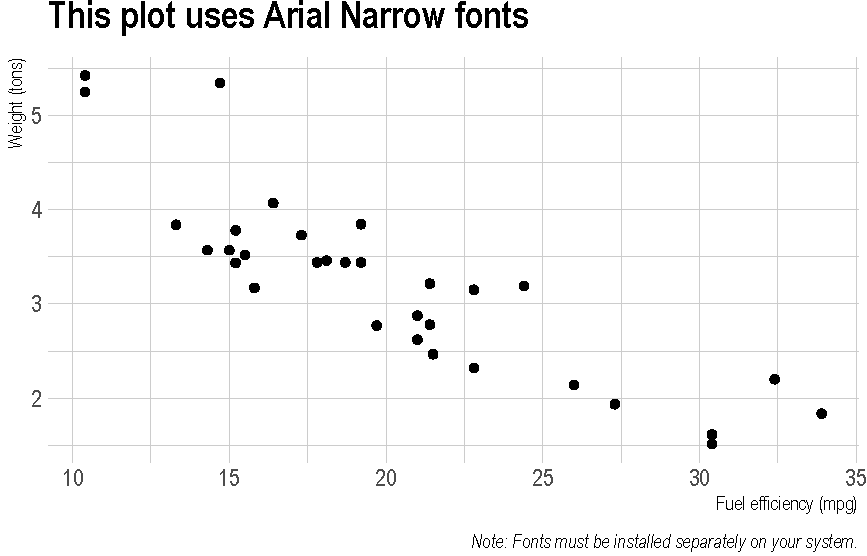
\includegraphics{Chapter1_files/figure-latex/mpg-1.pdf}

\hypertarget{ignore-interactive-content-when-exporting-to-pdf}{%
\subsubsection{Ignore interactive content when exporting to
PDF}\label{ignore-interactive-content-when-exporting-to-pdf}}

In general, this template tries to do a good job of automatically
handling (i.e.~ignoring) interactive content when exporting to PDF. A
notable exception is with embedded interactive content like external
GIFs. In this case, rather than typing the usual, say,
\texttt{!{[}{]}(mind-blown.gif)} directly in the Rmd file, you should
include the figure with \texttt{knitr::include\_graphics} in an R chunk.
This will allow you to control whether it renders, conditional on output
format. For example, the following chunk will render an actual GIF when
the knit target is HTML format, versus a message when that target is PDF
format.

\begin{verbatim}
## Sorry, this GIF is only available in the the HTML version of the notes.
\end{verbatim}

\end{document}
